\documentclass[12pt]{ctexart} 


\usepackage{subfigure}
\usepackage[graphicx]{realboxes}
\usepackage{listings}
\usepackage{xcolor}
\usepackage{amsmath}

% (1) choose a font that is available as T1
\usepackage{lmodern}
% (2) specify encoding
\usepackage[T1]{fontenc}
% (3) load symbol definitions
\usepackage{textcomp}

\usepackage{hyperref}

\usepackage{graphicx}


\hypersetup{hidelinks,
	colorlinks=true,
	allcolors=black,
	pdfstartview=Fit,
	breaklinks=true}


\definecolor{mygrey}{rgb}{0.945,0.945,0.945}
\definecolor{myred}{rgb}{1, 0.49, 0.63}
\definecolor{myblue}{rgb}{0,0.36, 0.67}

\lstset{
breaklines=true,
 basicstyle=\fontspec{Consolas},
 columns=fixed,       
 numbers=left,                                        % 在左侧显示行号
 numberstyle=\tiny\color{gray},                       % 设定行号格式
 frame=none,                                          % 不显示背景边框
 backgroundcolor=\color[RGB]{245,245,244},            % 设定背景颜色
 keywordstyle=\color[RGB]{40,40,255},                 % 设定关键字颜色
 numberstyle=\footnotesize\color{darkgray},           
 commentstyle=\it\color[RGB]{0,96,96},                % 设置代码注释的格式
 stringstyle=\rmfamily\slshape\color[RGB]{128,0,0},   % 设置字符串格式
 showstringspaces=false,                              % 不显示字符串中的空格
 %language=python,                                        % 设置语言
}
%\def\inline{\lstinline[basicstyle=\fontspec{微软雅黑},keywordstyle={}]}

%opening
\title{滤波}
\author{Liam}
\date{\today}

\begin{document}

\maketitle
\section{一般滤波器}
\subsection{限幅滤波法}
\begin{itemize}
    \item 优点:克服偶然因素引起的脉冲干扰
    \item 缺点:无法抑制周期性干扰,平滑度差
    \item 方法: 
    \subitem 如果本次值与上一次值的绝对值差$\leq A$,则本次值有效。
    \subitem 反之则无效  
\end{itemize}
\begin{lstlisting}
int filter(int newvalue)
{
    if(((NewValue - Value) > FILTER_A) || ((Value - NewValue) > FILTER_A))
        return Value;
    else
        return NewValue;
}
\end{lstlisting}
\subsection{中位值滤波法}
\begin{itemize}
    \item 连续采样奇数N次,将样本按照大小排序,取中间值为有效值。
    \item 优点:能够克服偶然因素波动干扰,对变化缓慢的观察量有好的滤波效果
    \item 缺点:不适用快速变化的量。
\end{itemize}
\begin{lstlisting}
int filter(buffertype *to_filter_buf)
{
    // 采样值从小到大排列(冒泡法)
  for(j = 0; j < FILTER_N - 1; j++) {
    for(i = 0; i < FILTER_N - 1 - j; i++) {
      if(filter_buf[i] > filter_buf[i + 1]) {
        filter_temp = filter_buf[i];
        filter_buf[i] = filter_buf[i + 1];
        filter_buf[i + 1] = filter_temp;
      }
    }
  }
  return filter_buf[(FILTER_N - 1) / 2];
}
\end{lstlisting}

\subsection{算术平均滤波法}
\begin{itemize}
    \item 优点:适用于具有随机干扰信号的滤波,适用于信号一般在某一值上下波动。
    \item 缺点:测量数据过慢或者过快的实时控制不好。
\end{itemize}
\begin{lstlisting}
    int filter(sometype data)
    {
        static sometype filter_sum = 0;
        for(int i=0; i<FILER_N,i++)
        {
            filter_sum += data;
        }
        return (int)(filter_sum / FILTER_N);
    }
\end{lstlisting}

\subsection{消抖滤波法}
\begin{itemize}
    \item 优点:对变化缓慢的被测量具有较好的滤波效果
    \item 作用:避免在临界值附近反复跳动or抖动。
    \item 缺点: 对于快速变化的量不适用
    \item 方法:
    \subitem 1. 设置一个滤波计数器,将每次采样的值和当前有效值进行对比
    \subitem 2. 如果采样值=当前有效值,则计数器清零;如果采样值<>当前有效值,则计数器+1,并判断计数器是否>=上限N(溢出);
    \subitem 3. 如果计数器溢出,则将本次值替换当前有效值,并清计数器。
\end{itemize}
\begin{lstlisting}
    
int Filter_Value;
int Value;

#define FILTER_N 12
int i = 0;
int Filter() {
  int new_value;
  new_value = Get_AD();
  if(Value != new_value) {
    i++;
    if(i > FILTER_N) {
      i = 0;
      Value = new_value;
    }
  }
  else
    i = 0;
  return Value;
}

\end{lstlisting}
\section{贝叶斯滤波}
\subsection{概率往事}
\subsubsection{随机变量}
定义在样本空间$\Omega$ 上的实值函数:
\begin{equation}
    X = X(\omega)
\end{equation}
被称为\textbf{随机变量} (random variable)。$\omega$表示样本空间$\Omega$里的随机事件,可能与数量有关(如传感器随机测得的前方障碍物的距离值,随机掷骰子得到的点数),也可能与数量无关(如随机掷硬币的结果可能为正面或反面)。
随机变量表示随机试验各种结果的实值单值函数。随机事件不论与数量是否直接有关,都可以数量化,即都能用数量化的方式表达。
\par
~\\
\textbf{离散型随机变量}:如果随机变量的函数值是实数轴上孤立的点
\begin{figure}[h]
    \centering
    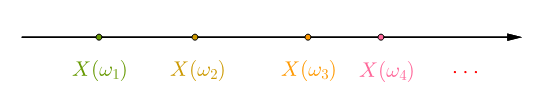
\includegraphics[width = 10cm]{image/640.png}
\end{figure}
\par
~\\
\textbf{连续型随机变量}:随机变量的函数值是实数轴上某个区间上所有的值
\begin{figure}[h]
    \centering
    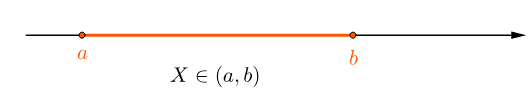
\includegraphics[width = 10cm]{image/1.png}
\end{figure}
~\\
\textbf{累积分布函数}:
\par
设$X$是一个随机变量,如果$\exists x$,则:
\begin{equation}
    F(x) = P(X\leq x )
\end{equation}
为随机变量的\textbf{累计分布函数}(Cumulative Distribution Function,CDF),又称概率分布函数,简称分布函数。
\\若 X 为离散型随机变量,存在函数$f_X(x)$,使其分布函数满足:
\begin{equation}
    F(x) = P(X\leq x)=\sum_{u\leq x}f_X(u)
\end{equation}
若 X 为连续型随机变量,存在函数$f_X(x)$,使其分布函数满足:
\begin{equation}
    F(x) = P(X\leq x)=\int_{-\infty}^{x}f_X(u)
\end{equation}
并且函数满足:
\begin{itemize}
    \item 单调性
    \item 有界性
    \item 右连续性
\end{itemize}
\par
\textbf{概率质量函数}
假设X为离散型随机变量,其全部可能取值为$x_1,x_2,\dots$,其概率分布列可表述为:

则称:
\begin{equation}
        f_X(x) = \left\{
            \begin{aligned}
            & p(x)=P  x\in \{x_i\},i=1,2,3, \\
            & 0 
        \end{aligned}
        \right.
\end{equation}
概率质量函数表征了离散型随机变量在各特定取值上的概率,满足:
\begin{itemize}
    \item 非负性
    \item 规范性
    \item 可加性
\end{itemize}
离散型随机变量概率质量函数的叠加得到了离散型随机变量的累积分布函数。
~\\
\textbf{概率密度函数}
\par
设$x$为连续型随机变量,存在函数$f_X(x)$,满足:
\begin{itemize}
    \item 非负性
    \item 规范和可加性
\end{itemize}
\[
  \in_{-\infty}^{\infty}f_X(x)dx = 1  
\]
则称函数为连续型随机变量X 的概率密度函数(Probability Density Function,PDF),连续型随机变量概率密度函数的积分得到了连续型随机变量的累积分布函数。

概率密度函数表征了连续型随机变量的输出值在某个确定的取值点附近的可能性。连续型随机变量的输出值在某个确定的取值点上的概率为0,但并不代表该事件不会发生。

\subsubsection{联合概率}
\textcolor{myblue}{\textbf{二维离散型随机变量的联合概率质量函数}}
若二维离散型随机变量(X,Y)所有可能的取值:
\begin{equation}
    (x_i,y_j),i,j = 1,2,3,\dots
\end{equation}
且存在函数$fx,y(x,y)$:
\begin{equation}
    f_{x,y}(x,y)=p(x,y)=P(X=x,Y=y), (x,y)\in \{x_i,y_i\},i,j=1,2,3,\dots
\end{equation}
则函数满足以下性质:
\begin{itemize}
    \item 非负性
    \item 规范和可加性
\end{itemize}
则称函数为$(x,y)$的\textbf{联合概率质量函数},又称联合分布列,此定义可以推广到多为离散随机变量。

二维离散型随机变量联合概率质量函数的叠加得到了二维离散型随机变量的联合累积分布函数:
\begin{equation}
    F_{X,Y}(x,y) = P(X\leq x,Y\leq y)=\sum_{u\leq x}\sum_{v\leq y}f_{X,Y}(u,v)
\end{equation}

\textcolor{myblue}{\textbf{二维连续型随机变量的联合概率密度函数}}
若对于随机变量$(X,Y), \exists f_{X,Y}(x,y)$满足:
满足:规范和可加性$\int_{-\infty}^{\infty}\int_{-\infty}^{\infty}f_{X,Y}(x,y)dxdy = 1$,非负性
则称函数为联合概率密度函数(Joint Probability Density Function),此定义可以推广到多维连续型随机变量。

二维连续型随机变量联合概率密度函数的积分得到了二维连续型随机变量的联合累积分布函数


\subsubsection{边缘概率}
\textcolor{myblue}{\textbf{二维离散型随机变量的边缘概率质量函数}}
若对于二维离散型随机变量(X,Y)所有可能的取值为$(x_i,y_j),i,j=1,2,3,\dots$
且联合概率质量函数$f_{X,Y}(x,y)$为:
\begin{equation}
    f_{x,y}(x,y)=p(x,y)=P(X=x,Y=y), (x,y)\in \{x_i,y_i\},i,j=1,2,3,\dots
\end{equation}
对$j$求和所得的函数:
\begin{equation}
    f_Y(y)=\sum_{i=1}^{\infty}f_{X,Y}(x_i,y)=\sum_{i=1}^{\infty}P(X=x_i,Y=y)=P(Y=y),y\in{y_i},j=1,2,3,\dots
\end{equation}
称为Y 的边缘概率质量函数(Marginal Probability Mass Function),又称边缘分布列。

二维离散型随机变量边缘概率质量函数的叠加得到了二维离散型随机变量的边缘累积分布函数(Marginal Cumulative Distribution Function):
\begin{equation}
    \begin{array}{rl}
        & F_X(x)=P(X\leq x)=\sum_{u\leq x}f_x(u)=\sum_{u\leq x}\sum_{j=1}P(X=u,Y=y_i)=  \\
        \sum_{u<x}P(X=u) \\
        & F_Y(y)=P(Y\leq y)=\sum_{v\leq y}f_y(v)=\sum_{v\leq y}\sum_{i=1}P(X=x_i,Y=v)= \\
        \sum_{u<x}P(Y=v)
    \end{array}
\end{equation}

\subsubsection{条件概率}
\textcolor{myblue}{二维离散型随机变量的条件概率质量函数}
若(x,y)是二维离散型随机变量,对于固定的$j$,若P(Y=y\textunderscore i)>0,则称为:
\begin{equation}
    f_{X|Y}(x|y)=P(X=x|Y=y)=\frac{P(X=x,Y=y)}{P(Y=y)}=\frac{f_{x,y}(x,y)}{f_X(x)},(x,y)\in\{x_i,y_j\},i,j=1,2,3,\dots
\end{equation}
为$X=x$条件下离散型随机变量 X 的条件概率质量函数。

简言之,对于二维离散型随机变量:
\begin{figure}[h]
    \centering
    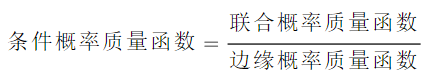
\includegraphics[width = 10cm]{image/2.png}
\end{figure}
二维离散型随机变量条件概率质量函数的叠加得到了二维离散型随机变量的条件累积分布函数(Conditional Cumulative Distribution Function):
\begin{equation}
    f_{X|Y}(x|y)=P(X\leq x | Y=y)=\sum_{u\leq x}f_{X|Y}(u|y)=\sum_{u\leq x}\frac{f_{x,y}(x,y)}{f_Y(y)}
\end{equation}

\textcolor{myblue}{二维连续型随机变量的条件概率密度函数}

假设二维连续型随机变量$(x,y)$的联合概率密度函数为$f_{x,y}(x,y)$,若对于固定的$Y=y$,有边缘概率密度函数$f_Y(y)>0$,则称函数:
\begin{equation}
    f_{X|Y}(x,y)=\frac{f_{x,y}(x,y)}{f_Y(y)}
\end{equation}
为随机变量 X 在条件下的条件概率密度函数(Conditional Probability Density Function)。
\begin{figure}[h]
    \centering
    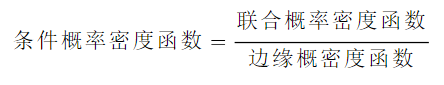
\includegraphics[width = 10cm]{image/3.png}
\end{figure}
二维连续型随机变量条件概率密度函数的积分得到了二维连续型随机变量的条件累积分布函数:
\begin{equation}
    F_{X|Y}(x|y) = P(X\leq x| Y = y)=\int_{-\infty}^{x}f_{X|Y}(u|y)du=\int_{-\infty}^{x}\frac{f_{X|Y}(u,y)}{f_Y(y)}du
\end{equation}



\subsubsection{全概率}
\textcolor{myblue}{二维离散型随机变量的全概率公式}


\textcolor{myblue}{二维连续型随机变量的全概率公式}
已知条件概率质量函数:
\begin{equation}
    f_{X|Y}(x|y)=\frac{f_{x,y}(x,y)}{f_Y(y)}
    f_{Y|X}(y|x)=\frac{f_{x,y}(x,y)}{f_X(x)}
\end{equation}
容易得到二维连续型随机变量联合概率密度函数的等价形式:
\begin{equation}
    f_{X,Y}(x,y) = f_{X|Y}(x|y)f_Y(y)=f_{Y|X}(y|x)f_X(x)
\end{equation}
由边缘概率密度函数与联合概率密度函数间的数量关系,得到二维连续型随机变量的全概率公式:
\begin{equation}
    f_X(x)=\int_{-\infty}^{\infty}f_{X|Y}(x|y)f_Y(y)dy
\end{equation}


\subsubsection{随机过程}
\textbf{随机过程}是定义在$\Omega × T$ 上的二元函数$X(\omega,t)$, 简单定义为一组随机变量的集合,即指定一参数集 $T$(又称指标集,通常为时间集),其中:
\begin{itemize}
    \item 对于固定的时间 t,$X(w,t)$为随机变量,简记为$X(t)$或 $X_t$
    \item 对于固定的 $w$(即固定每一时刻对应的随机变量的取值),$X(\omega,t)$为时间 t 的一般函数,称为样本函数(Sample Function)或样本轨道(Sample Path),简记为$x(t)$。随机过程也可定义为一组样本函数的集合。
\end{itemize}

注意:随机变量$X(t)$或$X_t$并不是时间 t 的函数,它只表示所有样本函数图片在 t 时刻的取值。

依据随机变量和参数集的连续离散情况,随机过程有以下四种类型:
\begin{itemize}
    \item 连续型随机过程:随机变量连续,参数连续;
    \item 离散型随机过程:随机变量离散,参数连续;
    \item 连续型随机序列:随机变量连续,参数离散;
    \item 离散型随机序列:随机变量离散,参数离散。
\end{itemize}

不同于确定过程,随机过程中的随机变量彼此间不独立。应该理解,贝叶斯滤波处理的是一个随机过程,
而且往往是一个连续型随机过程。

\subsection{贝叶斯公式}
\textcolor{myblue}{二维离散型随机变量的贝叶斯公式}
对于二维离散型随机变量$(x,y)$,由其条件概率质量函数与全概率公式,容易得到其贝叶斯公式:
\begin{equation}
    f_{X|Y}(x|y)=\frac{f_{X,y}(x,y)}{f_Y(y)}=\frac{f_{Y|X}(y|x)f_x(x)}{\sum_{i=1}^{\infty}f_{Y|X}(y|x_i)f_X(x_i)}
\end{equation}
\textcolor{myblue}{二维连续型随机变量的贝叶斯公式}
\begin{equation}
    f_{X|Y}(x|y)=\frac{f_{X,y}(x,y)}{f_Y(y)}=\frac{f_{Y|X}(y|x)f_x(x)}{\int_{i=1}^{\infty}f_{Y|X}(y|x_i)f_X(x_i)}
\end{equation}
二维连续型随机变量的条件累积分布函数推导:
\begin{figure}[h]
    \centering
    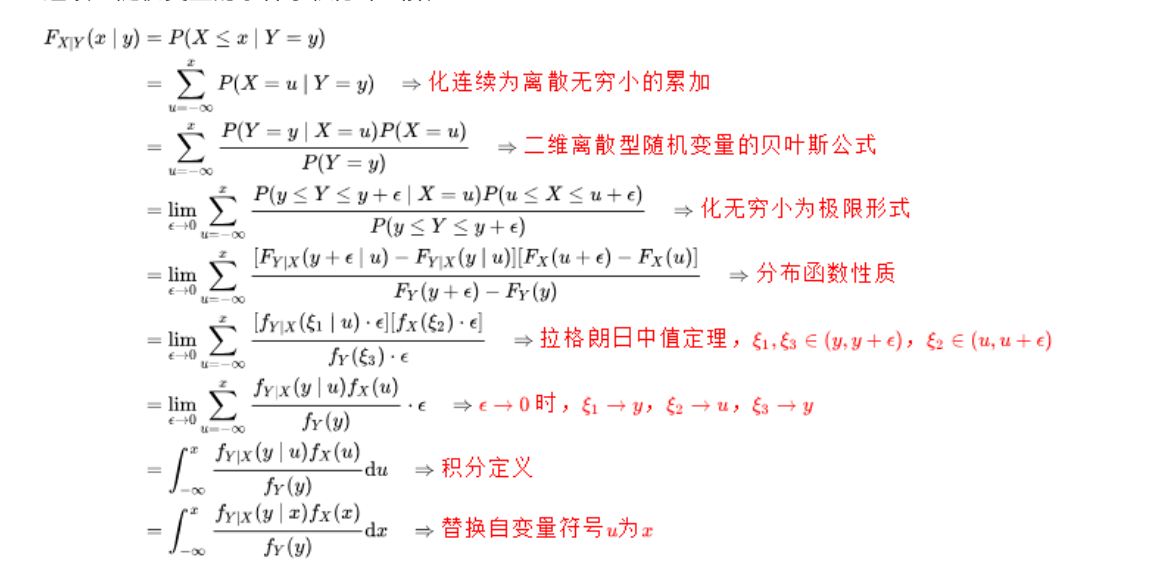
\includegraphics[width = 12cm]{image/4.png}
\end{figure}

\subsubsection{先验概率、似然概率与后验概率}
在二维连续型随机变量的贝叶斯公式中,有如下定义:
\begin{itemize}
    \item $f_X(x)$被称为先验概率密度(Prior Probability Density),表示根据以往的经验和分析,在本次试验或采样前便可获得的随机变量 X 的概率密度;
    \item $f_{Y|X}(y|x)$ 被称为似然概率密度(Likelihood Probability Density),表示在状态随机变量 X 取值为 x 的条件下,观测随机变量 Y 取值为 y 的概率密度,状态为因,观测为果,即由因推果;
    \item $f_{X|Y}(x|y)$被称为后验概率密度(Posterior Probability Density),表示在观测随机变量 Y 取值为 y 的条件下,状态随机变量 X 取值为 x 的概率密度,状态为因,观测为果,即由果推因。
    \item 当$y$为定值的时候,$\mu= \displaystyle \big[ \int_{-\infty}^{+\infty}f_{Y|X}(y|x)f(x)dx \big]^{-1}$,为常数,常被称为贝叶斯公式的\textbf{归一化常数}。
\end{itemize}

\subsubsection{似然概率}
上文中提到,似然概率密度函数$f_{Y|X}(y|X)$表示在状态随机变量 X 取值为 X 的条件下,观测随机变量 Y  取值为 y 的概率密度。似然概率密度函数表征了传感器检测精度,对于给定的状态条件 $X=x$,观测结果 $Y=y$的概率分布通常有三种模型:

(1) 等可能型

观测值在状态量真值附近呈均匀分布,此时的似然概率密度函数为常数。

(2) 阶梯型

观测值在状态量真值附近呈阶梯分布,此时的似然概率密度函数为分段常数。

(3) 正态分布型

观测值在状态量真值附近呈高斯分布,此时的似然概率密度函数为高斯函数:$\displaystyle f_{Y|X}(y|x) = \frac{1}{\sigma \sqrt{2\pi}}e^{-\frac{(y-x)^2}{2{\sigma}^2}}$

若假定似然概率密度函数为高斯函数,此时,似然概率密度函数的均值 x 代表状态量真值,$\sigma$代表传感器检测精度范围。若同时假定先验概率密度函数为高斯函数,即
\begin{equation}
    f_X(x) \sim N(\mu_1,{\sigma_1}^2), f_{Y|X}(y|x)\sim N(\mu_2,{\sigma_2}^2)
\end{equation}

后验概率密度函数方差既小于先验概率密度函数方差,也小于似然概率密度函数方差,系统不确定度降低.

\subsubsection{贝叶斯滤波推导}

\textcolor{myblue}{问题建模} 
(1) 问题描述

对于某状态量随机变量 X,从初始时刻 0 开始,对其进行观测,得到 $0 ~ k$ 时刻的观测值:

\begin{equation}
    y_0, y_1, y_2, \cdots , y_k \\
\end{equation}

求解 k 时刻状态量随机变量 $X_k$ 的最优估计 $\hat{x}_k$。

(2) 求解思路

以贝叶斯公式为求解方向,将问题转化为求解状态量随机变量 $X_k$ 后验概率密度函数的期望:

\begin{equation}
    \hat{x}_k=E[f_{X_k}^+(x)] \\
\end{equation}

进而需要求解状态量随机变量$ X_k$ 的先验概率密度函数与似然概率密度函数。我们认为,k 时刻的状态量随机变量 $X_k$ 与且仅与上一时刻的状态量随机变量 $X_{k-1}$ 有关,k 时刻的观测量随机变量 $Y_k$ 与且仅与 k 时刻的状态量随机变量$ X_k$ 有关,其中的数量关系我们分别称之为状态方程与观测方程:
\begin{equation}
    \begin{cases} X_k=f(X_{k-1})+Q_k \quad \Rightarrow \color{red}{状态方程} \\ Y_k=h(X_k)+R_k \quad \Rightarrow \color{red}{观测方程} \end{cases} \\
\end{equation}

f(x) 被称为状态转移函数,h(x) 被称为观测函数。

对于 0 时刻的初始状态量随机变量 $X_0$,认为观测值 $y_0$ 即为其真值,其后验概率密度函数即为其先验概率密度函数。我们可以根据经验知识(建模精度和传感器精度)写出 0 时刻的初始状态量随机变量 $X_0$ 的后验概率密度函数 $f_{X_0}^+(x)$、k 时刻过程噪声随机变量 $Q_k$ 的概率密度函数 $f_{Q_k}(x)$ 和 k 时刻观测噪声随机变量 $R_k$ 的概率密度函数 $f_{R_k}(x)$。

\textbf{符号定义}

1. 各时刻的状态量随机变量
$X_0, X_1, X_2, \cdots , X_k \\$
2. 各时刻的观测量随机变量
$Y_0, Y_1, Y_2, \cdots , Y_k \\$
3. 各时刻的观测值
$y_0, y_1, y_2, \cdots , y_k \\$
4. 各时刻的过程噪声随机变量
$Q_1, Q_2, \cdots , Q_k \\$
5. 各时刻的观测噪声随机变量
$R_1, R_2, \cdots , R_k \\$
6. 各时刻的过程噪声随机变量概率密度函数
$f_{Q_1}(x), f_{Q_2}(x), \cdots , f_{Q_k}(x) \\$
7. 各时刻的观测噪声随机变量概率密度函数
$f_{R_1}(x), f_{R_2}(x), \cdots , f_{R_k}(x) \\$
8. 各时刻的状态量随机变量先验概率密度函数
$f_{X_0}^-(x), f_{X_1}^-(x), f_{X_2}^-(x), \cdots , f_{X_k}^-(x) \\$
9. 各时刻的状态量随机变量后验概率密度函数
$f_{X_0}^+(x), f_{X_1}^+(x), f_{X_2}^+(x), \cdots , f_{X_k}^+(x) \\$
10. 各时刻状态量随机变量与观测量随机变量的似然概率密度函数

$f_{Y_1|X_1}(y_1 \ | \ x), f_{Y_2|X_2}(y_2 \ | \ x), \cdots , f_{Y_k|X_k}(y_k \ | \ x) \\$

\textbf{重要假设}

$X_0$ 分别与 $Q_1$, $Q_2$, $\cdots$ , $Q_k$ 相互独立;
$X_0$ 分别与 $R_1$, $R_2$, $\cdots$ , $R_k$ 相互独立;
$X_{k-1}$ 与 $Q_k$ 相互独立;
$X_{k}$ 与 $R_k$ 相互独立。
(5) 重要定理

条件概率里的条件可以作逻辑推导。例如:
\begin{equation}
P(X=1 \ | \ Y=2,Z=3)=P(X+Y=3 \ | \ Y=2,Z=3)=P(X+Y=3 \ | \ Y=2,Z-Y=1)
\end{equation}

预测步推导
已知 0 时刻状态量随机变量 $X_0$ 的后验概率密度函数 $f_{X_0}^+(x)$,状态转移函数 $f(x)$,1 时刻过程噪声随机变量 $Q_1$ 的概率密度函数 $f_{Q_1}(x)$,求解 1 时刻状态量随机变量 $X_1$ 的先验概率密度函数 $f_{X_1}^-(x)$。

类似二维连续型随机变量贝叶斯公式的推导过程,我们从求解 $X_1$ 的先验累积分布函数 $F_{X_1}^-$ 入手。

\begin{equation}
    \begin{aligned} F_{X_1}^-(x) & = P(X_1 \le x) \\ & = \sum_{u=-\infty}^xP(X_1=u) \quad \Rightarrow \color{red}{化连续为离散无穷小的累加} \\ & = \sum_{u=-\infty}^x\sum_{v=-\infty}^{+\infty}P(X_1=u \ | \ X_0=v)P(X_0=v) \quad \Rightarrow \color{red}{全概率公式} \\ & = \sum_{u=-\infty}^x\sum_{v=-\infty}^{+\infty}P[X_1-f(X_0)=u-f(v) \ | \ X_0=v]P(X_0=v) \quad \Rightarrow \color{red}{条件概率里的条件可以作逻辑推导} \\ & = \sum_{u=-\infty}^x\sum_{v=-\infty}^{+\infty}P[Q_1=u-f(v) \ | \ X_0=v]P(X_0=v) \quad \Rightarrow \color{red}{状态方程} \\ & = \sum_{u=-\infty}^x\sum_{v=-\infty}^{+\infty}P[Q_1=u-f(v)]P(X_0=v) \quad \Rightarrow \color{red}{X_{k-1}与Q_k相互独立} \\ & = \sum_{u=-\infty}^x\left\{\lim_{\epsilon \to 0}\sum_{v=-\infty}^{+\infty}f_{Q_1}[u-f(v)]·\epsilon · f_{X_0}^+(v)·\epsilon \right\} \quad \Rightarrow \color{red}{类似二维连续型随机变量贝叶斯公式的推导过程,将点概率化为概率密度与无穷小的乘积} \\ & = \sum_{u=-\infty}^x\left\{\lim_{\epsilon \to 0}\int_{-\infty}^{+\infty}f_{Q_1}[u-f(v)]f_{X_0}^+(v)\mathrm{d}v·\epsilon \right\} \quad \Rightarrow \color{red}{积分定义} \\ & = \int_{-\infty}^x \int_{-\infty}^{+\infty}f_{Q_1}[u-f(v)]f_{X_0}^+(v)\mathrm{d}v\mathrm{d}u \quad \Rightarrow \color{red}{积分定义} \\ & = \int_{-\infty}^x \int_{-\infty}^{+\infty}f_{Q_1}[x-f(v)]f_{X_0}^+(v)\mathrm{d}v\mathrm{d}x \quad \Rightarrow \color{red}{替换自变量符号u为x} \end{aligned} \\
\end{equation}

故,1 时刻状态量随机变量 $X_1$ 的先验概率密度函数为:

\begin{equation}
    f_{X_1}^-(x)=\frac{\mathrm{d}F_{X_1}^-(x)}{\mathrm{d}x}=\int_{-\infty}^{+\infty}f_{Q_1}[x-f(v)]f_{X_0}^+(v)\mathrm{d}v \\
\end{equation}

推导完毕。可以发现,先验概率密度函数本质来源于状态方程。

2.4.3 更新步推导
已知 1 时刻观测量随机变量$ Y_1$ 的取值$ y_1$,求解 1 时刻状态量随机变量与观测量随机变量的似然概率密度函数 $f_{Y_1|X_1}(y_1 \ | \ x)$,并联合预测步得到的 1 时刻状态量随机变量 $X_1$ 的先验概率密度函数 $f_{X_1}^-(x)$,求解 1 时刻状态量随机变量 $X_1$ 的后验概率密度函数 $f_{X_1}^+(x)$。

首先,求解似然概率密度函数 \(f_{Y_1|X_1}(y_1 | x)\):

\begin{equation}
\begin{aligned}
f_{Y_1|X_1}(y_1 | x) & =\lim_{\epsilon \to 0}\frac{F_{Y_1 | X_1}(y_1+\epsilon | x)-F_{Y_1 | X_1}(y_1 | x)}{\epsilon} \quad \Rightarrow \color{red}{\text{导数的定义}} \\
& =\lim_{\epsilon \to 0}\frac{P(y_1 \le Y_1 \le y_1 + \epsilon | X_1=x)}{\epsilon} \quad \Rightarrow \color{red}{\text{累积分布函数的性质}} \\
& =\lim_{\epsilon \to 0}\frac{P[y_1-h(x) \le Y_1-h(X_1) \le y_1 - h(x) + \epsilon | X_1=x]}{\epsilon} \quad \Rightarrow \color{red}{\text{条件概率里的条件可以作逻辑推导}} \\
& =\lim_{\epsilon \to 0}\frac{P[y_1-h(x) \le R_1 \le y_1 - h(x) + \epsilon | X_1=x]}{\epsilon} \quad \Rightarrow \color{red}{\text{观测方程}} \\
& =\lim_{\epsilon \to 0}\frac{P[y_1-h(x) \le R_1 \le y_1 - h(x) + \epsilon]}{\epsilon} \quad \Rightarrow \color{red}{X_{k}\text{与}R_k\text{相互独立}} \\
& =\lim_{\epsilon \to 0}\frac{F_{R_1}[y_1 - h(x) + \epsilon]-F_{R_1}[y_1 - h(x)]}{\epsilon} \quad \Rightarrow \color{red}{\text{累积分布函数的性质}} \\
& =f_{R_1}[y_1-h(x)] \quad \Rightarrow \color{red}{\text{导数的定义}}
\end{aligned}
\end{equation}

可以发现,似然概率密度函数本质来源于观测方程。

然后,联合预测步得到的 1 时刻状态量随机变量 \(X_1\) 的先验概率密度函数 \(f_{X_1}^-(x)\),求解 1 时刻状态量随机变量 \(X_1\) 的后验概率密度函数 \(f_{X_1}^+(x)\):

\begin{equation}
f_{X_1}^+(x)=\eta_1·f_{Y_1|X_1}(y_1 | x)·f_{X_1}^-(x)=\eta_1·f_{R_1}[y_1-h(x)]·f_{X_1}^-(x)
\end{equation}

其中,归一化常数 \(\eta_1\) 为:

\begin{equation}
\eta_1=\left[\int_{-\infty}^{+\infty}f_{Y_1|X_1}(y_1 | x)f_{X_1}^-(x)\mathrm{d}x\right]^{-1}=\left\{\int_{-\infty}^{+\infty}f_{R_1}[y_1-h(x)]f_{X_1}^-(x)\mathrm{d}x\right\}^{-1}
\end{equation}

推导完毕。

2.4.4 递推流程
由预测步和更新步的推导结果,可得到由 0 时刻状态量随机变量 \(X_0\) 的后验概率密度函数 \(f_{X_0}^+(x)\) 到 \(k\) 时刻状态量随机变量 \(X_k\) 的后验概率密度函数 \(f_{X_k}^+(x)\) 的递推流程:

\begin{equation}
\begin{aligned}
f_{X_0}^+(x) & \stackrel{\text{预测}}{\Longrightarrow} f_{X_1}^-(x)=\int_{-\infty}^{+\infty}f_{Q_1}[x-f(v)]f_{X_0}^+(v)\mathrm{d}v \stackrel{\text{观测更新}}{\Longrightarrow} f_{X_1}^+(x)=\eta_1·f_{R_1}[y_1-h(x)]·f_{X_1}^-(x) \\
& \stackrel{\text{预测}}{\Longrightarrow} f_{X_2}^-(x)=\int_{-\infty}^{+\infty}f_{Q_2}[x-f(v)]f_{X_1}^+(v)\mathrm{d}v \stackrel{\text{观测更新}}{\Longrightarrow} f_{X_2}^+(x)=\eta_2·f_{R_2}[y_2-h(x)]·f_{X_2}^-(x) \\
& \cdots \\
& \stackrel{\text{预测}}{\Longrightarrow} f_{X_k}^-(x)=\int_{-\infty}^{+\infty}f_{Q_k}[x-f(v)]f_{X_{k-1}}^+(v)\mathrm{d}v \stackrel{\text{观测更新}}{\Longrightarrow} f_{X_k}^+(x)=\eta_k·f_{R_k}[y_k-h(x)]·f_{X_k}^-(x)
\end{aligned}
\end{equation}

其中,归一化常数 \(\eta_k\) 为:

\begin{equation}
\eta_k=\left\{\int_{-\infty}^{+\infty}f_{R_k}[y_k-h(x)]f_{X_k}^-(x)\mathrm{d}x\right\}^{-1}
\end{equation}

最终,可得到 \(k\) 时刻状态量随机变量 \(X_k\) 的最优估计 \(\hat{x}_k\):

\begin{equation}
\hat{x}_k=E[f_{X_k}^+(x)]=\int_{-\infty}^{+\infty}xf_{X_k}^+(x)\mathrm{d}x
\end{equation}

\par
~\\
\textcolor{myblue}{完整算法框架}

(1) 设初值

初始 0 时刻状态量随机变量 \(X_0\) 的后验概率密度函数:

\[f_{X_0}^+(x)\]

(2) 预测步

\(k\) 时刻状态量随机变量 \(X_k\) 的先验概率密度函数:

\[f_{X_k}^-(x)=\int_{-\infty}^{+\infty}f_{Q_k}[x-f(v)]f_{X_{k-1}}^+(v)\mathrm{d}v\]

(3) 更新步

\(k\) 时刻状态量随机变量 \(X_k\) 的后验概率密度函数:

\[f_{X_k}^+(x)=\eta_k·f_{R_k}[y_k-h(x)]·f_{X_k}^-(x)\]

归一化常数 \(\eta_k\):

\[\eta_k=\left\{\int_{-\infty}^{+\infty}f_{R_k}[y_k-h(x)]f_{X_k}^-(x)\mathrm{d}x\right\}^{-1}\]

(4) 求解状态量后验估计

\(k\) 时刻状态量随机变量 \(X_k\) 的后验估计:

\[\hat{x}_k^+=E[f_{X_k}^+(x)]=\int_{-\infty}^{+\infty}xf_{X_k}^+(x)\mathrm{d}x\]

2.5 贝叶斯滤波的缺点及解决方法
2.5.1 缺点
从上文的推导及结论中可以发现,求解预测步中的先验概率密度函数 \(f_{X_k}^-(x)\)、更新步中的归一化常数 \(\eta_k\)、最终的最优估计 \(\hat{x}_k\) 时均涉及到无穷积分,而大多数情况无法得到解析解,使得贝叶斯滤波算法的直接应用十分困难。

2.5.2 解决办法
为了解决贝叶斯滤波中的无穷积分问题,通常从两个角度出发:

(1) 作理想假设

假设状态转移函数 \(f(x)\) 和观测函数 \(h(x)\) 均为线性函数,过程噪声随机变量 \(Q_k\) 和 观测噪声随机变量 \(R_k\) 均服从均值为 0 的正态分布——卡尔曼滤波(Kalman Filter)
假设状态转移函数 \(f(x)\) 和(或)观测函数 \(h(x)\) 为非线性函数,过程噪声随机变量 \(Q_k\) 和 观测噪声随机变量 \(R_k\) 均服从均值为 0 的正态分布——扩展卡尔曼滤波(Extended Kalman Filter)和无迹卡尔曼滤波(Unscented Kalman Filter)
(2) 化连续为离散

将无穷积分转化为数值积分,一般有以下方法:

\begin{itemize}
    \item 高斯积分(不常用)
    \item 蒙特卡罗积分(粒子滤波,Particle Filter)
    \item 直方图滤波
\end{itemize}



\section{高斯滤波}
高斯滤波,称为\textbf{一个重要的递归状态估计器家族}
\subsection{卡尔曼滤波}
\textbf{卡尔曼滤波}是以贝叶斯滤波为理论基础,并通过假设状态量随机变量(以下简称状态量)、
观测量均服从\textbf{正态分布},假设过程噪声、观测噪声均服从均值为 0 的正态分布,以及假设\textbf{状态转移函数和观测函数均为线性函数},
实现对连续型随机过程的递推状态估计。简言之,卡尔曼滤波是在贝叶斯滤波框架下求解线性高斯问题。

\par
简单来讲,卡尔曼滤波器就是根据上一时刻的状态,预测当前时刻的状态,
将预测的状态量与当前时刻的观测量进行加权,加权后的结果才认为是当前实际的状态量,而非仅听信当前的观测量。

\subsubsection{卡尔曼滤波的假设}
卡尔曼滤波以贝叶斯滤波为理论基础,并作了六个前提假设:
~//
(1) 假设一:状态量服从正态分布
\[
X \sim \mathcal{N}(\mu_X, \ \sigma_X^2) \\
\]
(2) 假设二:观测量服从正态分布
\[
Y \sim \mathcal{N}(\mu_Y, \ \sigma_Y^2) \\
\]
(3) 假设三:过程噪声服从均值为 0 的正态分布
\[
Q \sim \mathcal{N}(0, \ \sigma_Q^2) \\
\]
(4) 假设四:观测噪声服从均值为 0 的正态分布
\[
Q \sim \mathcal{N}(0, \ \sigma_R^2) \\
\]
(5) 假设五:状态转移函数为线性函数
\[
f(X_k)=F*X_{k-1}+B*u_k \\
\]
其中,F 为状态转移比例项,对于单一状态量的卡尔曼滤波中,F 为一常数;B 为控制比例项,$u_k$ 为控制量,B 和 $u_k$ 的乘积可视为线性状态转移函数中的截距项。在简单的系统中,常常没有控制项 B 和 $u_k$。


\subsubsection{矩阵形式的卡尔曼滤波}
当状态量和观测量不再是单一的随机变量而是由多个随机变量组成的序列时,卡尔曼滤波中各个量的维数也将随之改变:
\[
    \begin{aligned}
    & \text{1. 状态量 } X  \text{由随机变量演变为随机向量,随机向量中的每一个分量为一个状态量} \\ 
    & \text{随机变量。维数为 } n_X \times 1 \\
    & \text{2. 状态转移比例项 } F  \text{演变为矩阵,维数为 } n_X \times n_X \\
    & \text{3. 控制量 } u_k  \text{演变为矩阵,维数为 } n_u \times 1 \\
    & \text{4. 控制比例项 } B  \text{演变为矩阵,维数为 } n_X \times n_u \\
    & \text{5. 状态量概率密度函数均值 } \mu  \text{演变为矩阵,维数为 } n_X \times 1 \\
    & \text{6. 状态量概率密度函数方差 } \sigma^2  \text{演变为协方差矩阵,用 } \Sigma \text{ 表示,维数为 } n_X \times n_X \\
    & \text{7. 过程噪声方差 } {\sigma_Q}^2  \text{演变为协方差矩阵,用 } \Sigma_Q \text{ 表示,维数为 } n_X \times n_X \\
    & \text{8. 观测量 } Y  \text{由随机变量演变为随机向量,随机向量中的每一个分量为一个观测量} \\
    & \text{随机变量。维数为 } n_Y \times 1 \\
    & \text{9. 观测值 } y_k  \text{由单一值演变为由单一值组成的值矩阵,维数为 } n_Y \times 1 \\
    & \text{10. 观测比例项 } H  \text{演变为矩阵,维数为 } n_Y \times n_X \\
    & \text{11. 观测噪声方差 } {\sigma_R}^2  \text{演变为协方差矩阵,用 } \Sigma_R \text{ 表示,维数为 } n_Y \times n_Y \\
    & \text{12. 卡尔曼增益系数 } K  \text{演变为矩阵,维数为 } n_X \times n_Y 
    \end{aligned}
\]  
~\\
        对应的五个公式演变为:
        
\begin{align}
    \mu_k^- &= F*\mu_{k-1}^++B*u_k \tag{4.1} \\
    \Sigma_k^- &= F*\Sigma_{k-1}^+*F^T+{\Sigma_{Q_k}} \tag{4.2} \\
    \mu_k^+ &= \mu_k^-+K*(y_k-H*\mu_k^-) \tag{4.3} \\
    \Sigma_k^+ &= (I-K*H)*\Sigma_k^- \tag{4.4} \\
    K &= \Sigma_k^-*H^T*(H*\Sigma_k^-*H^T+{\Sigma_{R_k}})^{-1} \tag{4.5}
\end{align}
        
公式 (4.3) 中 $\mu_k^+$ 即 k 时刻状态量 $X_k$ 的后验估计 $\hat{x}_k^+,y_k-H*\mu_k^- $常被称为残差(Residual)或新息(Innovation);
公式 (4.4) 中的 I 代表单位矩阵,维数为 $n_X \times n_X$。
        
从结果中还可以发现,外部控制项$ B*u_k $通过影响先验估计均值间接影响了后验估计均值,但对后验估计方差没有影响。


\subsubsection{实战写卡尔曼滤波器}
\textcolor{myblue}{简单例子:}
假设有个小车在道路上向右侧匀速运动,我们在左侧安装了一个测量小车距离和速度传感器,传感器每1秒测一次小车的位置s和速度v,如下图所示:
\begin{figure}[h]
    \centering
    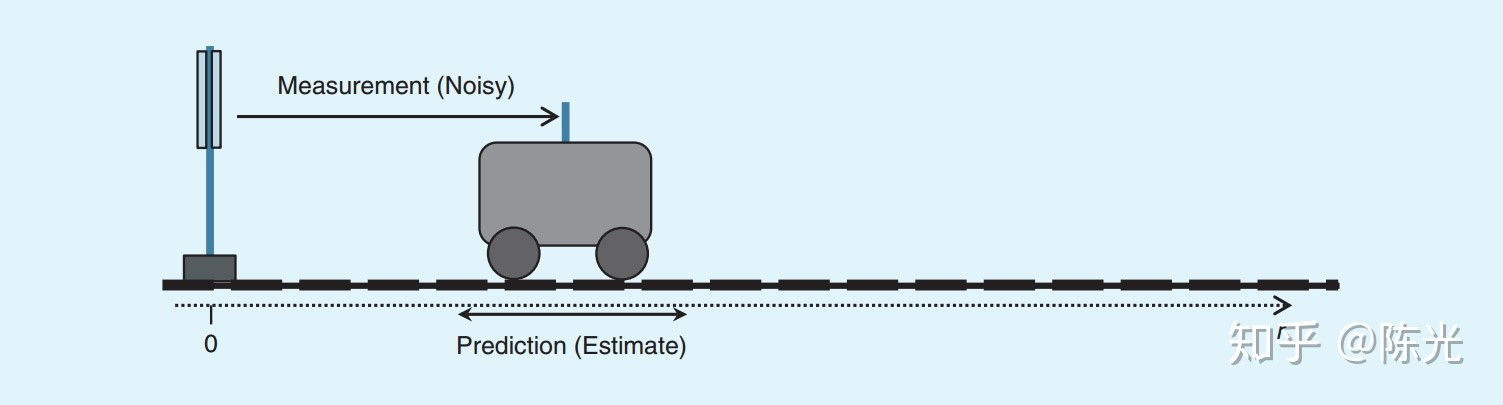
\includegraphics[width = 12cm]{image/11.jpg}
\end{figure}
我们用向量xt来表示当前小车的状态,该向量也是最终的输出结果,被称作状态向量(state vector):
\[
    x_t=
    \left[ 
        \begin{matrix}
            s_t \\
            v_t 
        \end{matrix}
    \right] \tag{1}
\]
由于测量误差的存在,传感器无法直接获取小车位置的真值,只能获取在真值附近的一个近似值,
可以假设测量值在真值附近服从高斯分布。如下图所示,测量值分布在红色区域的左侧或右侧,真值则在红色区域的波峰处。
\begin{figure}[h]
    \centering
    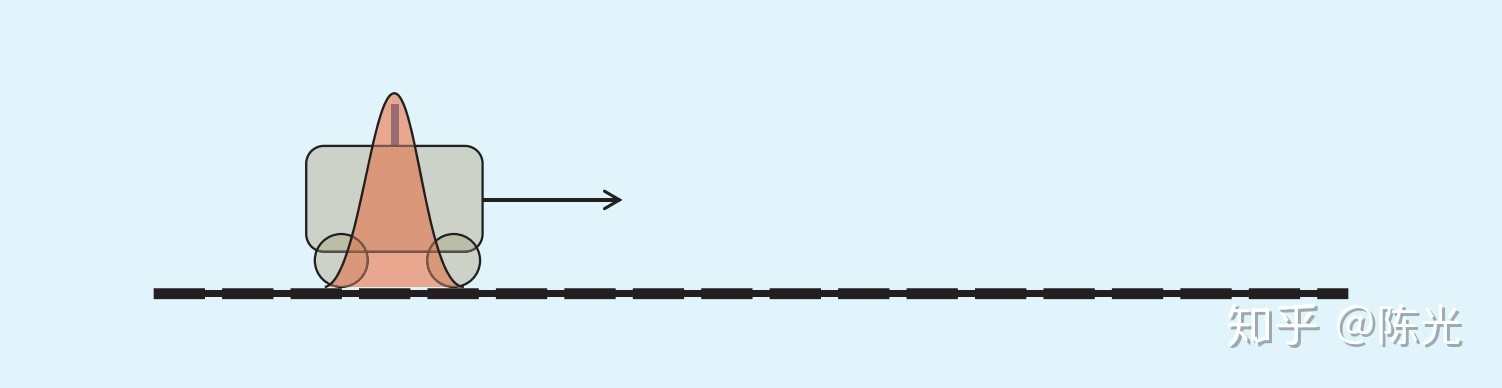
\includegraphics[width = 12cm]{image/12.jpg}
\end{figure}
由于是第一次测量,没有小车的历史信息,我们认为小车在1秒时的状态x与测量值z相等,表示如下:
\[
    x_t= 
    \left[
        \begin{matrix}
            s_1 \\
            v_1 
        \end{matrix}
    \right] \tag{2}
\]
公式中的1表示第1秒。
~\\
\textcolor{myblue}{预测}
\par
预测是卡尔曼滤波器中很重要的一步,这一步相当于使用历史信息对未来的位置进行推测。
根据第1秒小车的位置和速度,我们可以推测第2秒时,小车所在的位置应该如下图所示。
会发现,图中红色区域的范围变大了,这是因为预测时加入了速度估计的噪声,是一个放大不确定性的过程。
\begin{figure}[h]
    \centering
    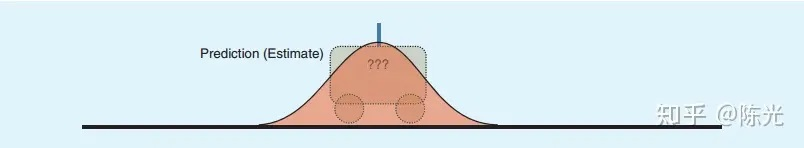
\includegraphics[width = 12cm]{image/13.jpg}
\end{figure}
根据小车第一秒的状态进行预测,得到预测的状态xpre:
\[
    x_{pre}= 
    \left[
        \begin{matrix}
            s_1+v_1 \\
            v_1 
        \end{matrix}
    \right] \tag{2}
\]
其中,pre是prediction的简称;时间间隔为1秒,所以预测位置为距离+速度*1;由于小车做的是匀速运动,因此速度保持不变。

\textcolor{myblue}{观测}
在第2秒时,传感器对小车的位置做了一次观测,我们认为小车在第2秒时观测值为z2,用向量表示第2秒时的观测结果为:
\[
    z_2= 
    \left[
        \begin{matrix}
            s_2 \\
            v_2 
        \end{matrix}
    \right] \tag{2}
\]
很显然,第二次观测的结果也是存在误差的,我们将预测的小车位置与实际观测到的小车位置放到一个图上,即可看到:
\begin{figure}[h]
    \centering
    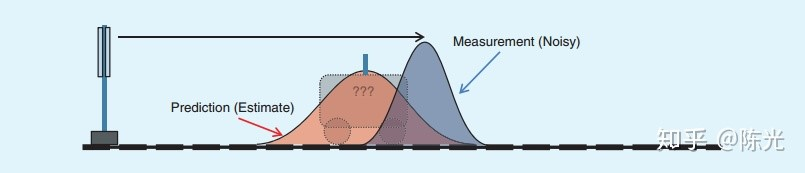
\includegraphics[width = 12cm]{image/14.jpg}
\end{figure}
图中红色区域为预测的小车位置,蓝色区域为第2秒的观测结果。

很显然,这两个结果都在真值附近。为了得到尽可能接近真值的结果,我们将这两个区域的结果进行加权,取加权后的值作为第二秒的状态向量。

为了方便理解,可以将第2秒的状态向量写成:
\[
x_2=w_1 \times x_{pre} +w_2\times Z_2  
\]
其中,w1为预测结果的权值,w2为观测结果的权值。两个权值的计算是根据预测结果和观测结果的不确定性来的,
这个不确定性就是高斯分布中的方差的大小,方差越大,波形分布越广,不确定性越高,这样一来给的权值就会越低。

加权后的状态向量的分布,可以用下图中绿色区域表示:
\begin{figure}[h]
    \centering
    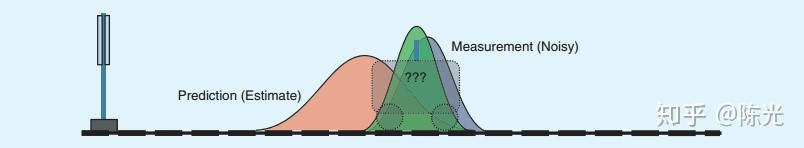
\includegraphics[width = 12cm]{image/15.jpg}
\end{figure}
你会发现绿色区域的方差比红色区域和蓝色区域的小。这是因为进行加权运算时,需要将两个高斯分布进行乘法运算,得到的新的高斯分布的方差比两个做乘法的高斯分布都小。

两个不那么确定的分布,最终得到了一个相对确定的分布,这是卡尔曼滤波的一直被推崇的原因。
~\\
\textcolor{myblue}{再预测,再观测(Prediction \& Measurement)}

第1秒的初始化以及第2秒的预测、观测,实现卡尔曼滤波的一个周期。

同样的,我们根据第2秒的状态向量做第3秒的预测,再与第3秒的观测结果进行加权,就得到了第3秒的状态向量;再根据第3秒的状态向量做第4秒的预测,再与第4秒的观测结果进行加权,就得到了第4秒的状态向量。以此往复,就实现了一个真正意义上的卡尔曼滤波器。

以上就是卡尔曼滤波器的感性分析过程,下面我们回归理性,谈谈如何将以上过程写成代码。
\begin{figure}[p]
    \centering
    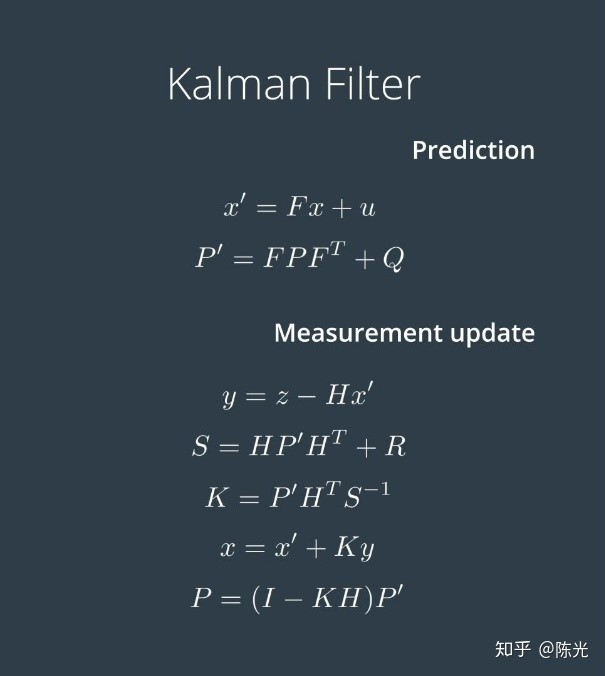
\includegraphics[width = 15cm]{image/16.jpg}
    \caption{七个描述卡尔曼滤波器的公式}
\end{figure}

\begin{lstlisting}

\end{lstlisting}







\subsubsection{扩展卡尔曼滤波}
\textbf{扩展卡尔曼滤波}(Extended Kalman Filter,EKF)是标准卡尔曼滤波在\textbf{非线性情形}下的一种扩展形式,
它是一种高效率的递归滤波器(自回归滤波器)。
\par
EKF 的基本思想是利用泰勒级数展开将非线性系统的状态转移函数 
和(或)观测函数 线性化,然后采用卡尔曼滤波框架对信号进行滤波,因此它是一种次优滤波。
~\\
\textcolor{myblue}{\textbf{与卡尔曼滤波相同的假设}}

(1) 假设一:状态量服从正态分布
\[
X \sim \mathcal{N}(\mu_X, \ \sigma_X^2) \\
\]
(2) 假设二:观测量服从正态分布
\[
Y \sim \mathcal{N}(\mu_Y, \ \sigma_Y^2) \\
\]
(3) 假设三:过程噪声服从均值为 0 的正态分布
\[
Q \sim \mathcal{N}(0, \ \sigma_Q^2) \\
\]
(4) 假设四:观测噪声服从均值为 0 的正态分布
\[
R \sim \mathcal{N}(0, \ \sigma_R^2) \\
\]

\textcolor{myblue}{\textbf{与卡尔曼滤波不同的假设}}
(5) 假设五:状态转移函数和(或)观测函数为非线性函数

在卡尔曼滤波的前提假设中,认为状态方程中的状态转移函数 f(x) 以及观测方程中的观测函数 h(x) 均为线性函数。基于这种线性假设,
存在常数或常矩阵 F,使得 f(x) 可以写成卡尔曼滤波中的线性形式,存在常数或常矩阵 H,使得 h(x) 也可以写成卡尔曼滤波中的线性形式。

不同于标准卡尔曼滤波,\textbf{扩展卡尔曼滤波处理的是非线性系统},假设系统的状态转移函数和(或)观测函数为非线性函数。
~\\
\textcolor{myblue}{\textbf{矩阵形式的扩展卡尔曼滤波}}
状态转移比例项
\[
    F_j= \begin{pmatrix} \frac{\partial f_1}{\partial X_{k-1}^1} & \frac{\partial f_1}{\partial X_{k-1}^2} & \cdots & \frac{\partial f_1}{\partial X_{k-1}^{n_X}} \\ \frac{\partial f_2}{\partial X_{k-1}^1} & \frac{\partial f_2}{\partial X_{k-1}^2} & \cdots & \frac{\partial f_2}{\partial X_{k-1}^{n_X}} \\\vdots & \vdots & \ddots & \vdots \\\frac{\partial f_{n_X}}{\partial X_{k-1}^1} & \frac{\partial f_{n_X}}{\partial X_{k-1}^2} & \cdots & \frac{\partial f_{n_X}}{\partial X_{k-1}^{n_X}} \end{pmatrix} \Bigg|_{X_{k-1}=\hat{X}_{k-1}^+} \\    
\]
观测比例项
\[
    H_j= \begin{pmatrix} \frac{\partial h_1}{\partial X_k^1} & \frac{\partial h_1}{\partial X_k^2} & \cdots & \frac{\partial h_1}{\partial X_k^{n_X}} \\ \frac{\partial h_2}{\partial X_k^1} & \frac{\partial h_2}{\partial X_k^2} & \cdots & \frac{\partial h_2}{\partial X_k^{n_X}} \\ \vdots & \vdots & \ddots & \vdots \\\frac{\partial h_{n_Y}}{\partial X_k^1} & \frac{\partial h_{n_Y}}{\partial X_k^2} & \cdots & \frac{\partial h_{n_Y}}{\partial X_k^{n_X}}\end{pmatrix} \Bigg|_{X_k=\hat{X}_k^-} \\
\]

五个公式:
\begin{align}
    \mu_k^- & = f(\mu_{k-1}^+) \tag{4.1} \\
    \Sigma_k^- & = F_j*\Sigma_{k-1}^+*F_j^T+{\Sigma_{Q_k}} \tag{4.2} \\
    \mu_k^+ & = \mu_k^-+K*[y_k-h(\mu_k^-)] \tag{4.3} \\
    \Sigma_k^+ & = (I-K*H_j)*\Sigma_k^- \tag{4.4} \\
    K & =\Sigma_k^-*H_j^T*(H_j*\Sigma_k^-*H_j^T+{\Sigma_{R_k}})^{-1} \tag{4.5}   
\end{align} 
公式 (4.3) 中 $\mu_k^+$ 即 k 时刻状态量 $X_k$ 的后验估计 $\hat{x}_k^+$,$y_k-h(\mu_k^-)$ 常被称为残差(Residual)或新息(Innovation);
公式 (4.4) 中的 I 代表单位矩阵,维数为 $n_X \times n_X$。

当然,对于某个非线性系统,不一定状态转移和观测都是非线性的:
\begin{itemize}
    \item 线性的状态转移 + 非线性的观测
    此时,滤波递推公式由卡尔曼滤波的预测步两公式和扩展卡尔曼滤波的更新步三公式组成。
    \item 非线性的状态转移 + 线性的观测
    此时,滤波递推公式由扩展卡尔曼滤波的预测步两公式和卡尔曼滤波的更新步三公式组成。
\end{itemize}
\end{document}
